\documentclass[12pt,a4paper]{report}
\usepackage[french]{babel}
\usepackage[utf8]{inputenc}
\usepackage[T1]{fontenc}
\usepackage{graphicx}
\usepackage{fancyhdr}
\usepackage{geometry}
\usepackage{setspace}
\usepackage{titlesec}
\usepackage{hyperref}
\usepackage{amsmath} % Add this line to import the amsmath package
\usepackage{amsmath} % Add this line to import the necessary package

\geometry{left=2.5cm, right=2.5cm, top=2.5cm, bottom=2.5cm}
\titleformat{\chapter}[hang]{\huge\bfseries}{\thechapter}{2pc}{}
\onehalfspacing




% Configuration des En-têtes et Pieds de page
\pagestyle{fancy}
\fancyhf{} % Clear all headers and footers

% Images en en-tête
\fancyhead[L]{
\includegraphics[width=1.5cm]{logo_chalmers.jpg}} % Image en en-tête gauche
\fancyhead[R]{
\includegraphics[width=1.5cm]{logo_chalmers.jpg}} % Image en en-tête droite


% Numérotation des pages en pied de page au centre
\fancyfoot[C]{\thepage}

% Pour éviter les en-têtes et pieds de page par défaut des chapitres
\fancypagestyle{plain}{
    \fancyhf{}
    \fancyhead[L]{
\includegraphics[width=3cm]{logo_chalmers.jpg}}
    \fancyhead[R]{
\includegraphics[width=1.2cm]{logo_x.png}}
    \fancyfoot[C]{\thepage}
}



\begin{document}


% Page de Garde
\begin{titlepage}
    \begin{center}
        \vspace*{1cm}
        
        \Huge
        \textbf{Comparing forecast performance on different synthetic pandemics }
        
        \vspace{0.5cm}
        \LARGE
        Sous-titre du Rapport
        
        \vspace{1.5cm}
        
        \textbf{Grégoire Béchade}
        
        \vfill
        
        \Large
        Rapport de stage effectué chez \\
        Nom de l'Entreprise
        
        \vspace{0.8cm}
        
        \includegraphics[width=0.4\textwidth]{logo.png}
        
        \vfill
        
        \Large
        Under the direction of \\
        Philipp Gerlee
        
        \vspace{0.8cm}
        
        \Large
        Nom de l'Université \\
        Nom de la Faculté \\
        Nom du Département
        
    \end{center}
\end{titlepage}

% Page de Garde vide (optionnelle)
\newpage
\thispagestyle{empty}
\mbox{}
\newpage

% Table des matières
\tableofcontents
\newpage

% Introduction
\chapter*{Introduction}
\addcontentsline{toc}{chapter}{Introduction}

% Contenu des chapitres


\chapter{The data}


\chapter{Models}

\cite{ref1}

\section{SIRH model}


The SIRH model is a compartemental model used in epidemiology to model the spread a pandemic. 
This model splits the population in different compartments which represent the health conditions of the individuals.
The evolution of the pandemic is modelled by a system of differential equations.

Let $S_t$, $I_t$, $R_t$ and $H_t$ be the number of susceptible, infected, recovered and hospitalized individuals at time $t$.

The SIRH model is defined by this system of differential equations:\\


\begin{equation}
    \begin{cases}
        \frac{dS}{dt} & = - \beta \frac{S I}{N} \\
        \frac{dI}{dt} & = \beta \frac{S I }{N} - (\gamma_i + h) I \\
        \frac{dR}{dt} & = \gamma_i I + \gamma_h H  \\
        \frac{dH}{dt} & = h I - \gamma_h H  \\
    \end{cases}
\end{equation}
    



where $\beta$ is the transmission rate, $\gamma_i$ is the recovery rate, $\gamma_h$ is the hospitalization rate and $h$ is the hospitalization rate.
This model is useful for policymakers because of its explanatory power and its simplicity.
Moreover, the parameters of the model have a physical interpretation. 

\subsection{Computing confidence intervals with delta-method}

For many models, we did not have an explici way to compute the confidence interval of the prediction. 
We used the delta-method, which enables to output a confidence interval based on the error of estimation of the model associated with the estimation of the noise of the data. 

We suppose that the number of hospitalized at day $i$ follows the mode $h_{\theta^*}$: 
$ Y_i = h_{\theta^*}(i) + \epsilon_i$ where $\epsilon_i \sim \mathcal{N}(0, \sigma^2)$

Let $h_{\theta}(i)$ be the prediction of the model $h$, with parameters $\theta$ at time $i$, we have : \\
$ \hat{\theta} = argmin_{\theta} \sum_{i=1}^{n} (Y_i - h_{\theta}(i))^2$ be the least-squares estimator of $\theta^*$ \\



if we note : 
 $Y = 
\begin{pmatrix}
    Y_1 \\
    Y_2 \\
    \vdots \\
    Y_n
\end{pmatrix} $ \\[0.2cm]

and $h_{\theta} =
\begin{pmatrix}
    h_{\theta}(1) \\
    h_{\theta}(2) \\
    \vdots \\
    h_{\theta}(n)
\end{pmatrix} $ \\[0.2cm], 

we have : 

$\hat{\theta} = argmin_{\theta} ||Y - h_{\theta}||^2$ \\

We linearize around $\theta^*$ :
$h_{\theta}(i) \simeq h_{\theta^*}(i) +  (\theta - \theta^*)^T\nabla_{\theta} h_{\theta^*}(i)$ \\

We have :\\
$\hat{\theta} = argmin_{\theta} ||Y - h_{\theta^*} +  (\theta - \theta^*)^T\nabla_{\theta} h_{\theta^*}||^2$ \\







\begin{figure}
    \centering
    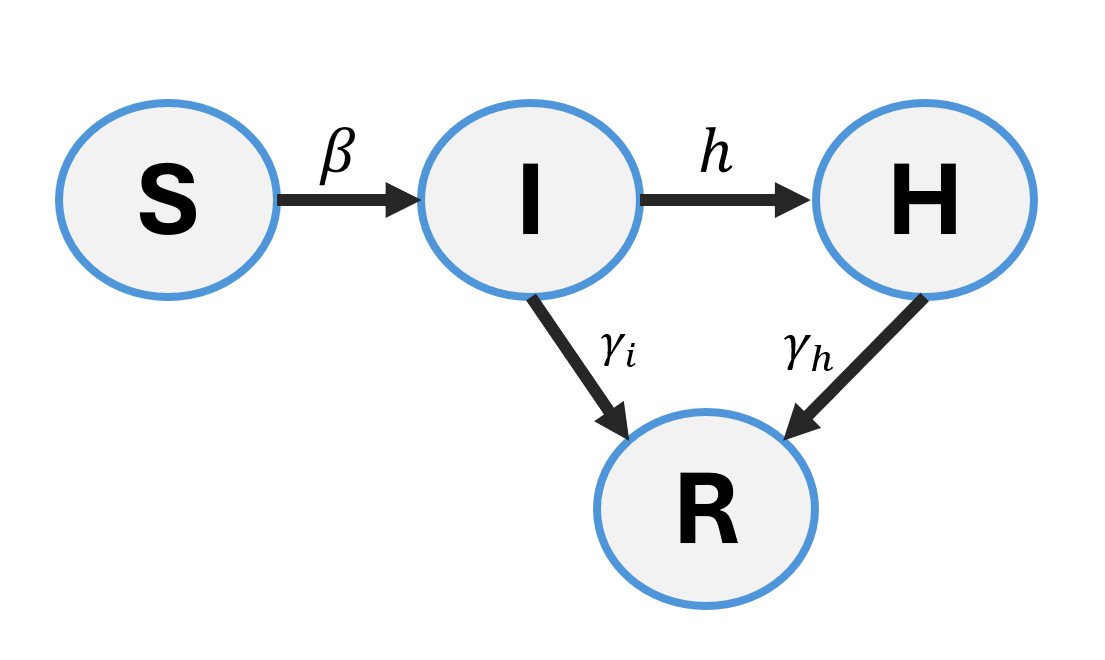
\includegraphics[width=0.5\textwidth]{SIRH_model.png}
    \caption{Scheme of the compartments of the SIRH model}
    \label{fig:sirh}
\end{figure}





\subsection{Titre de la Sous-section 1}



Contenu de votre rapport...

\chapter{Titre du Chapitre 2}
\section{Titre de la Section 2}

Contenu de votre rapport...

% Ajouter des images
\begin{figure}[h!]
    \centering
    
\includegraphics[width=0.5\textwidth]{logo_chalmers.jpg}
    \caption{Description de l'image}
    \label{fig:image1}
\end{figure}

% Conclusion
\chapter*{Conclusion}
\addcontentsline{toc}{chapter}{Conclusion}

Conclusion de votre rapport...

% Bibliographie
\newpage
\addcontentsline{toc}{chapter}{Bibliographie}
\bibliographystyle{plain}
\bibliography{bibliographie}

% Annexes
\appendix
\chapter{Titre de l'Annexe}

Contenu de l'annexe...

\pagestyle{plain}

\end{document}
